\let\negmedspace\undefined
\let\negthickspace\undefined
\documentclass[journal]{IEEEtran}
\usepackage[a5paper, margin=10mm, onecolumn]{geometry}
%\usepackage{lmodern} % Ensure lmodern is loaded for pdflatex
\usepackage{tfrupee} % Include tfrupee package

\setlength{\headheight}{1cm} % Set the height of the header box
\setlength{\headsep}{0mm}     % Set the distance between the header box and the top of the text

\usepackage{gvv-book}
\usepackage{gvv}
\usepackage{cite}
\usepackage{amsmath,amssymb,amsfonts,amsthm}
\usepackage{algorithmic}
\usepackage{graphicx}
\usepackage{textcomp}
\usepackage{xcolor}
\usepackage{txfonts}
\usepackage{listings}
\usepackage{enumitem}
\usepackage{mathtools}
\usepackage{gensymb}
\usepackage{comment}
\usepackage[breaklinks=true]{hyperref}
\usepackage{tkz-euclide} 
\usepackage{listings}
% \usepackage{gvv}                                        
\def\inputGnumericTable{}                                 
\usepackage[latin1]{inputenc}                                
\usepackage{color}                                            
\usepackage{array}                                            
\usepackage{longtable}                                       
\usepackage{calc}                                             
\usepackage{multirow}                                         
\usepackage{hhline}                                           
\usepackage{ifthen}                                           
\usepackage{lscape}
\begin{document}

\bibliographystyle{IEEEtran}
\vspace{3cm}

\title{11.16.3.16}
\author{EE24BTECH11021 - Eshan Ray}
% \maketitle
% \newpage
% \bigskip
{\let\newpage\relax\maketitle}

\renewcommand{\thefigure}{\theenumi}
\renewcommand{\thetable}{\theenumi}
\setlength{\intextsep}{10pt} % Space between text and floats


\numberwithin{equation}{enumi}
\numberwithin{figure}{enumi}
\renewcommand{\thetable}{\theenumi}

\textbf{Question:} Events E and F are such that P(not E or not F) = $0.25$, State whether E and F are mutually exclusive.\\
\solution{\\
\textbf{Theoretical Solution:}\\
    Given,\\
\begin{align}
    P\brak{E'+F'} &= 0.25
\end{align}
Using De-Morgan's Law, we get,
\begin{align}
    \brak{E'+F'}' &= \brak{EF}\\
    P\brak{\brak{E'+F'}} &= P\brak{EF}\\
    P\brak{EF} &= 1 - P\brak{E'+F'}\\
    P\brak{EF} &= 0.75\neq 0
\end{align}
Since, $P\brak{EF}\neq 0$ proving that the events $E$ and $F$ are not mutually exclusive.
\textbf{Computational Solution:}\\
Let $X_1$ be an indicator random variable of the event $\brak{E'+F'}$.\\
$X_1$ is defined as:
\begin{align}
	X_1 =
	\begin{cases}
		1 ,& \brak{E^\prime+F^\prime}\\
		0 ,& \brak{E^\prime+F^\prime}^\prime = EF \\
	\end{cases}
\end{align}
The PMF of the random variable $X_1$ is:
\begin{align}
	p_{X_1}(n) =
	\begin{cases}
		p_1 ,& n = 1\\
		1 - p_1 ,& n = 0
	\end{cases}
\end{align}
where,
\begin{align}
    p_1 = 0.25
\end{align}

\begin{figure}[ht]
    \centering
    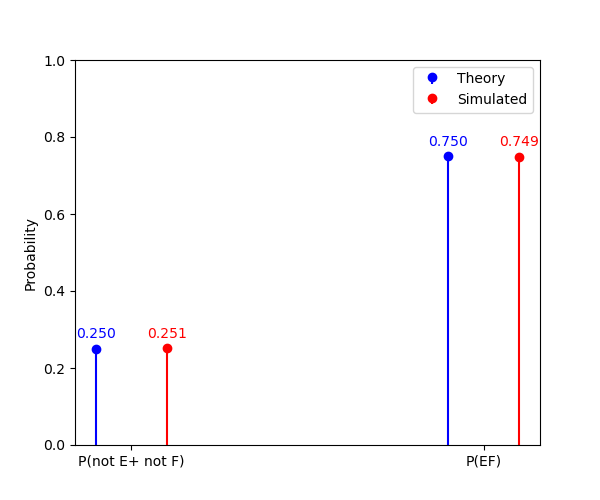
\includegraphics[width=\columnwidth]{plots/plot.png}
    \caption{Theoritical vs Simulation}
    \label{fig:Plot1}
\end{figure}
}

\end{document}

